\documentclass[]{article}
\usepackage{lmodern}
\usepackage{amssymb,amsmath}
\usepackage{ifxetex,ifluatex}
\usepackage{fixltx2e} % provides \textsubscript
\ifnum 0\ifxetex 1\fi\ifluatex 1\fi=0 % if pdftex
  \usepackage[T1]{fontenc}
  \usepackage[utf8]{inputenc}
\else % if luatex or xelatex
  \ifxetex
    \usepackage{mathspec}
  \else
    \usepackage{fontspec}
  \fi
  \defaultfontfeatures{Ligatures=TeX,Scale=MatchLowercase}
\fi
% use upquote if available, for straight quotes in verbatim environments
\IfFileExists{upquote.sty}{\usepackage{upquote}}{}
% use microtype if available
\IfFileExists{microtype.sty}{%
\usepackage{microtype}
\UseMicrotypeSet[protrusion]{basicmath} % disable protrusion for tt fonts
}{}
\usepackage[margin=1in]{geometry}
\usepackage{hyperref}
\hypersetup{unicode=true,
            pdftitle={Supplementary Material: Epigenomic prediction of cardiovascular risk and interactions with traditional risk metrics},
            pdfborder={0 0 0},
            breaklinks=true}
\urlstyle{same}  % don't use monospace font for urls
\usepackage{graphicx,grffile}
\makeatletter
\def\maxwidth{\ifdim\Gin@nat@width>\linewidth\linewidth\else\Gin@nat@width\fi}
\def\maxheight{\ifdim\Gin@nat@height>\textheight\textheight\else\Gin@nat@height\fi}
\makeatother
% Scale images if necessary, so that they will not overflow the page
% margins by default, and it is still possible to overwrite the defaults
% using explicit options in \includegraphics[width, height, ...]{}
\setkeys{Gin}{width=\maxwidth,height=\maxheight,keepaspectratio}
\IfFileExists{parskip.sty}{%
\usepackage{parskip}
}{% else
\setlength{\parindent}{0pt}
\setlength{\parskip}{6pt plus 2pt minus 1pt}
}
\setlength{\emergencystretch}{3em}  % prevent overfull lines
\providecommand{\tightlist}{%
  \setlength{\itemsep}{0pt}\setlength{\parskip}{0pt}}
\setcounter{secnumdepth}{0}
% Redefines (sub)paragraphs to behave more like sections
\ifx\paragraph\undefined\else
\let\oldparagraph\paragraph
\renewcommand{\paragraph}[1]{\oldparagraph{#1}\mbox{}}
\fi
\ifx\subparagraph\undefined\else
\let\oldsubparagraph\subparagraph
\renewcommand{\subparagraph}[1]{\oldsubparagraph{#1}\mbox{}}
\fi

%%% Use protect on footnotes to avoid problems with footnotes in titles
\let\rmarkdownfootnote\footnote%
\def\footnote{\protect\rmarkdownfootnote}

%%% Change title format to be more compact
\usepackage{titling}

% Create subtitle command for use in maketitle
\providecommand{\subtitle}[1]{
  \posttitle{
    \begin{center}\large#1\end{center}
    }
}

\setlength{\droptitle}{-2em}

  \title{Supplementary Material: Epigenomic prediction of cardiovascular risk and
interactions with traditional risk metrics}
    \pretitle{\vspace{\droptitle}\centering\huge}
  \posttitle{\par}
    \author{}
    \preauthor{}\postauthor{}
    \date{}
    \predate{}\postdate{}
  
\usepackage{booktabs}
\usepackage{longtable}
\usepackage{array}
\usepackage{multirow}
\usepackage{wrapfig}
\usepackage{float}
\usepackage{colortbl}
\usepackage{pdflscape}
\usepackage{tabu}
\usepackage{threeparttable}
\usepackage{threeparttablex}
\usepackage[normalem]{ulem}
\usepackage{makecell}
\usepackage{xcolor}

\usepackage{float}

\begin{document}
\maketitle

\newcommand{\beginsupplement}{
  \setcounter{table}{0}  
  \renewcommand{\thetable}{S\arabic{table}}
  \setcounter{figure}{0} 
  \renewcommand{\thefigure}{S\arabic{figure}}
}

\setcounter{table}{0}  
  \renewcommand{\thetable}{S\arabic{table}}
  \setcounter{figure}{0} 
  \renewcommand{\thefigure}{S\arabic{figure}}

\hypertarget{supplementary-methods}{%
\section{Supplementary Methods}\label{supplementary-methods}}

\hypertarget{womens-health-initiative}{%
\subsection{Women's Health Initiative}\label{womens-health-initiative}}

WHI methylation data came from the BA23 ancillary study, a combined
case-control and pseudo case-cohort sampling of 2129 women from the
Women's Health Initiative study. WHI is a larger prospective cohort
beginning in 1993 that included over 160,000 postmenopausal women from
across the United
States\textsuperscript{\protect\hyperlink{ref-Anderson1998}{1}}.
Included subjects had no self-reported CVD at baseline, and cases were
chosen based on incident centrally adjudicated angina,
revascularization, or CHD event during follow-up. Inclusion criteria for
methylation measurement resulted in an oversampling of African American
and Hispanic participants. Blood samples used for measurement of DNA
methylation and clinical biochemistry were taken at baseline. Data are
available in the dbGaP public repository (accession: phs000200.v11.p3;
downloaded on September 27, 2017).

\hypertarget{framingham-heart-study-offspring-cohort}{%
\subsection{Framingham Heart Study Offspring
Cohort}\label{framingham-heart-study-offspring-cohort}}

FHS methylation data came from a substudy of the Framingham Heart Study
that measured DNA methylation in 2726 subjects from the Offspring
Cohort. The Framingham Offspring Cohort was originally established in
1971 to follow 5209 children of the original Framingham Heart Study
participants and their
spouses\textsuperscript{\protect\hyperlink{ref-Kannel1979}{2}}. Fasting
blood samples for both methylation and clinical biochemistry were
collected from participants at Exam 8, which took place from 2005-8.
Blood samples were also provided for clinical biochemistry measurements
in previous exams, constituting the ``past exposures'' examined here.
Data are available in the dbGaP public repository (accession:
phs000007.v29.p10; downloaded on September 27, 2017). Adjudicated
cardiovascular event data was collected through 2015, and events were
defined here as any of: myocardial infarction, angina pectoris, stroke
(approximately 90\% being ischemic), or death from CHD (Framingham event
codes 1-29). FHS methylation data were collected in two primary batches
in two centers -- one in subjects from a nested case-control for CVD
measured at Johns Hopkins University
(FHS-JHU)\textsuperscript{\protect\hyperlink{ref-Joehanes2013}{3}}, and
the other in a larger set of remaining Framingham Offspring participants
measured at the University of Minnesota (FHS-UM).

\hypertarget{lothian-birth-cohorts}{%
\subsection{Lothian Birth Cohorts}\label{lothian-birth-cohorts}}

The Lothian Birth Cohorts consist of two birth cohorts (born in 1921 and
1936) established in the Lothian region of
Scotland\textsuperscript{\protect\hyperlink{ref-Deary2012}{4},\protect\hyperlink{ref-Taylor2018}{5}}.
Only the 1936 cohort was analyzed here. Blood samples were collected in
three waves starting in 2004, with our primary analyses here focusing on
samples from Wave 1 (2004-2007). Cardiovascular outcomes were defined as
general CVD or stroke determined at each wave, and event times for
survival models were approximated based on the time between Wave 1 and
the wave at which the event was reported. LBC data are accessible
through the European Genome-phenome Archive (accession:
EGAD00010000604).

\hypertarget{regicor}{%
\subsection{REGICOR}\label{regicor}}

The REGICOR dataset analyzed here consisted of a nested case-control for
myocardial infarction within the larger REGICOR (REgistre GIroní del
COR) cohort from the Girona Province in Catalonia (Spain). Whole blood
samples were collected from 391 total participants, with those from
cases generally collected within 24 hours of the event. Characteristics
for this population are available in Supp. Table S3.

\hypertarget{dna-methylation-data-processing}{%
\subsection{DNA methylation data
processing}\label{dna-methylation-data-processing}}

DNA methylation data for all initial cohorts (WHI, FHS, and LBC) were
collected using the Illumina HumanMethylation450 microarray
platform\textsuperscript{\protect\hyperlink{ref-Bibikova2011}{6}} and
downloaded as raw intensity files. Preprocessing was performed using the
\emph{minfi} and \emph{wateRmelon} packages for
R\textsuperscript{\protect\hyperlink{ref-Aryee2014}{7},\protect\hyperlink{ref-Pidsley2013}{8}}.
Sample-wise filters were as follows: robust overall signal in the main
cluster based on visual inspection of an intensity plot, less than 10\%
of probes undetected at a detection threshold of p\textless{}1e-16, and
a reported sex matching methylation-based sex prediction. Probes were
removed using the following criteria: more than 10\% of samples
undetected at a detection threshold of p\textless{}1e-16, location in
the X or Y chromosomes, non-CpG probes, cross-hybridizing probes, probes
measuring SNPs, and probes with an annotated SNP at the CpG site or in
the single-base extension region. Samples were normalized using the Noob
method for background correction and dye-bias normalization, followed by
the BMIQ method for probe type
correction\textsuperscript{\protect\hyperlink{ref-Fortin2016}{9},\protect\hyperlink{ref-Teschendorff2013}{10}}.
Blood cell fractions for 6 blood cell types (CD4+ T-cells, CD8+ T-cells,
B-cells, natural killer cells, monocytes, and granulocytes) were
estimated using a common reference-based
method\textsuperscript{\protect\hyperlink{ref-Houseman2012}{11}}, and 5
of these (excluding granulocytes) were included in cell count-adjusted
statistical models. After quality control and filtering steps, 390597
CpG sites were shared between the 3 datasets, formatted as beta values
(ratio of methylated signal to total microarray signal).

DNA methylation data for the REGICOR cohort were collected using the
Illumina MethylationEPIC microarray
platform\textsuperscript{\protect\hyperlink{ref-Pidsley2016}{12}} and
analyzed using the
\emph{wateRmelon}\textsuperscript{\protect\hyperlink{ref-Pidsley2013}{8}}
and methylumi\textsuperscript{\protect\hyperlink{ref-Davis2019}{13}} R
packages. Samples were excluded based on detection p-value
\textgreater{}0.05 in at least 1\% of probes or failure to cluster in
the appropriate sex based on X chromosome methylation. Probes were
excluded based on detection p-value \textgreater{}0.05 in at least 1\%
of samples, a bead count \textless{}3 in at least 5\% of samples,
discarding by Illumina based on underperformance (n=1,031) or changes in
the manufacturing process (n=977), non-CpG targets, and
cross-hybridization (n=43,979). A batch normalization was performed by
standardizing beta values to mean zero and unit variance within each
bisulfite conversion batch prior to analysis. After quality control and
preprocessing, 811,610 CpG sites across 391 individuals were available
for analysis. Participants were further excluded from analysis due to
unknown smoking habits (n=10) and unavailable information regarding
diabetes, hypertension, or hyperlipidemia (n=53). Surrogate variable
analysis\textsuperscript{\protect\hyperlink{ref-Leek2007}{14}} was used
to calculate two surrogate variables, representing potential technical
and biological confounders, for adjustment in MRS replication models.

\hypertarget{supplementary-tables-and-figures}{%
\section{Supplementary Tables and
Figures}\label{supplementary-tables-and-figures}}

\begin{ThreePartTable}
\begin{TableNotes}
\item[1] No covariates
\item[2] Adjusted for age, sex, and estimated cell type fractions
\item[3] Additionally adjusted for BMI, LDL, HDL, SBP, diabetes status, and current smoking
\item[4] Adjusted for Framingham Risk Score only
\end{TableNotes}
\begin{longtable}{lrl}
\caption{\label{tab:fhs-holdout-noPE}MRS performance in held-out FHS subset without past CVD events}\\
\toprule
Model & HR per s.d. MRS & p\\
\midrule
Unadjusted\textsuperscript{1} & 1.55 & 1.9e-08\\
Basic\textsuperscript{2} & 1.27 & 7.3e-03\\
Plus risk factors\textsuperscript{3} & 1.30 & 6.0e-03\\
FRS only\textsuperscript{4} & 1.37 & 7.7e-05\\
\bottomrule
\insertTableNotes
\end{longtable}
\end{ThreePartTable}

\newpage

\begin{longtable}{llrr}
\caption{\label{tab:stability}MRS stability as evaluated by using multiple within-subject measurements. Generic ICC heuristics for reference: 0-0.5 = poor, 0.5-0.75 = moderate, 0.75 - 0.9 = good, 0.9-1 = excellent.}\\
\toprule
Cohort & Group type & \# of pairs/groups & ICC\\
\midrule
FHS & Duplicates & 26 & 0.85\\
LBC36 & Samples over multiple visits & 758 & 0.68\\
LBC36 & Samples over subsequent visits (Wave 1 \& 2) & 758 & 0.69\\
LBC36 & Samples over longer time frame (Wave 1 \& 3) & 758 & 0.61\\
\bottomrule
\end{longtable}

\begin{longtable}{ll}
\caption{\label{tab:regicor-description}Description of REGICOR myocardial infarction nested case-control population (continuous variables presented as: mean (standard deviation)}\\
\toprule
Sample size & 391\\
Prior myocardial infarction & 50.1\%\\
Ancestry (\% European) & 100\%\\
Age & 63.2 (6.9)\\
Sex (\% female) & 48.6\\
Smoking & 21.5\%\\
Body mass index & 28.5 (4.8)\\
LDL cholesterol & 127 (26)\\
HDL cholesterol & 50.0 (10.5)\\
Systolic blood pressure & 135 (18)\\
Diabetes prevalence & 24.7\%\\
\bottomrule
\end{longtable}

\newpage

\begin{figure}[h]
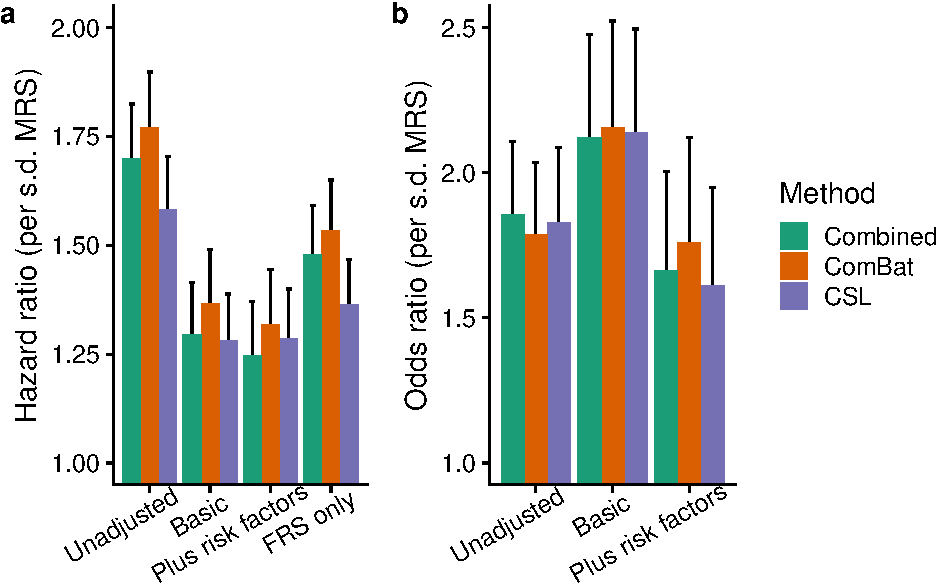
\includegraphics{figures/csl-comparison-1} \caption{Comparison of modeling approaches. Performance metrics are shown as a function of the test dataset, either FHS-UM (a) or REGICOR (b), and the covariate adjustment. Performance is quantified by either hazard ratio from Cox models (a) or odds ratio from logistic models (b). Covariate sets used for adjustment for models named here are identical to their descriptions for the regression models presented above. Errors bars represent standard errors for the hazard ratio or odds ratio estimates.}\label{fig:csl-comparison}
\end{figure}

\begin{longtable}{lrl}
\caption{\label{tab:risk-score-validation}Validation of Framingham Risk Score}\\
\toprule
Study & HR per s.d. MRS & p\\
\midrule
WHI & 1.50 & 4.7e-61\\
FHS-JHU & 1.40 & 9.9e-06\\
FHS-UM & 1.63 & 8.5e-22\\
LBC & 1.01 & 9.2e-01\\
\bottomrule
\end{longtable}

\newpage

\begin{figure}[h]
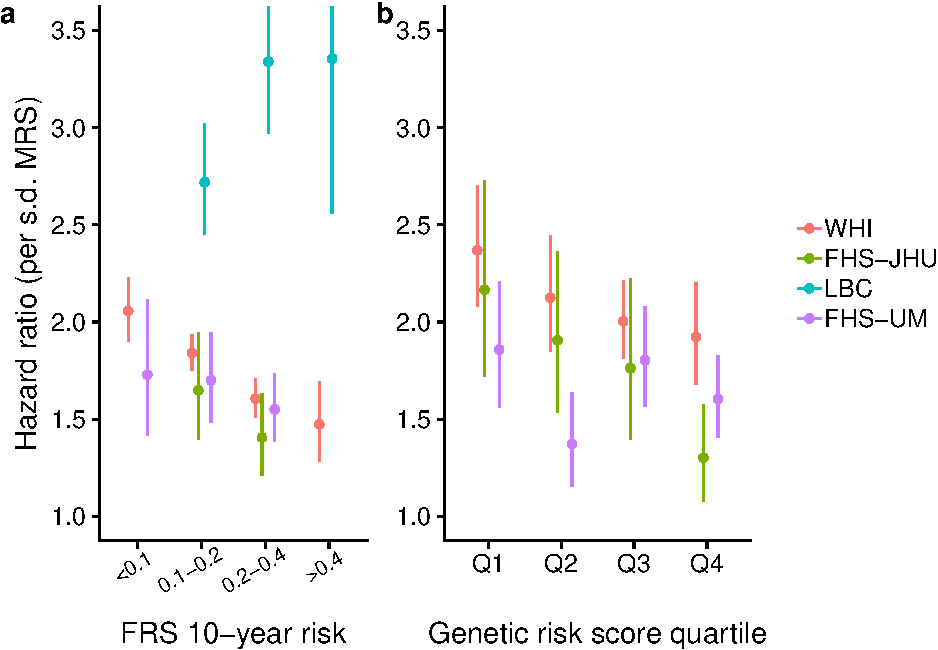
\includegraphics{figures/interactions-1} \caption{Interactions of MRS with other biomarkers of CVD risk. a) Hazard ratios for the MRS within subsets of 10-year generalized CVD risk according to the Framingham Risk Score. b) Hazard ratios for the MRS within quartiles of a genetic cardiovascular risk score (in white participants only for WHI). Hazard ratios are estimated using the final MRS, which was trained using each of these datasets. Stratum-specific Cox regressions were adjusted for age, sex, and estimated cell subtype fractions. Estimates for strata with less than 25 incident events are not shown. Error bars represent standard errors for the hazard ratio estimates (cut off above in panel (a) for ease of visualization of other points).}\label{fig:interactions}
\end{figure}

\begin{longtable}{llr}
\caption{\label{tab:regicor-interactions}Risk factor-stratified MRS performance in the REGICOR dataset}\\
\toprule
Risk factor group & OR per s.d. MRS [95\% CI] & N\\
\midrule
Q1 & 4.49 [1.64-12.28] & 119\\
Q2 & 1.17 [0.67-2.04] & 90\\
Q3 & 2.58 [1-6.68] & 60\\
Q4 & 1.2 [0.31-4.59] & 55\\
\bottomrule
\end{longtable}

\newpage

\hypertarget{supplementary-references}{%
\section*{Supplementary References}\label{supplementary-references}}
\addcontentsline{toc}{section}{Supplementary References}

\hypertarget{refs}{}
\leavevmode\hypertarget{ref-Anderson1998}{}%
1. Anderson GL, Cummings SR, Freedman LS, Furberg C, Henderson MM,
Johnson SR, et al. Design of the Women's Health Initiative Clinical
Trial and Observational Study. \emph{Controlled Clinical Trials}.
1998;19:61--109.

\leavevmode\hypertarget{ref-Kannel1979}{}%
2. Kannel WB, Feinleib M, Mcnamara PM, Garrison RJ, Castelli WP. An
investigation of coronary heart disease in families: The framingham
offspring study. \emph{American Journal of Epidemiology}.
1979;110:281--290.

\leavevmode\hypertarget{ref-Joehanes2013}{}%
3. Joehanes R, Ying S, Huan T, Johnson AD, Raghavachari N, Wang R, et
al. Gene Expression Signatures of Coronary Heart Disease.
\emph{Arteriosclerosis, Thrombosis, and Vascular Biology}.
2013;33:1418--1426.

\leavevmode\hypertarget{ref-Deary2012}{}%
4. Deary IJ, Gow AJ, Pattie A, Starr JM. Cohort Profile: The Lothian
Birth Cohorts of 1921 and 1936. \emph{International Journal of
Epidemiology}. 2012;41:1576--1584.

\leavevmode\hypertarget{ref-Taylor2018}{}%
5. Taylor AM, Pattie A, Deary IJ. Cohort Profile Update: The Lothian
Birth Cohorts of 1921 and 1936. \emph{International Journal of
Epidemiology}. 2018;47:1042--1042r.

\leavevmode\hypertarget{ref-Bibikova2011}{}%
6. Bibikova M, Barnes B, Tsan C, Ho V, Klotzle B, Le JM, et al. High
density DNA methylation array with single CpG site resolution.
\emph{Genomics}. 2011;98:288--295.

\leavevmode\hypertarget{ref-Aryee2014}{}%
7. Aryee MJ, Jaffe AE, Corrada-Bravo H, Ladd-Acosta C, Feinberg AP,
Hansen KD, et al. Minfi: A flexible and comprehensive Bioconductor
package for the analysis of Infinium DNA methylation microarrays.
\emph{Bioinformatics}. 2014;30:1363--1369.

\leavevmode\hypertarget{ref-Pidsley2013}{}%
8. Pidsley R, Y Wong CC, Volta M, Lunnon K, Mill J, Schalkwyk LC. A
data-driven approach to preprocessing Illumina 450K methylation array
data. \emph{BMC Genomics}. 2013;14:293.

\leavevmode\hypertarget{ref-Fortin2016}{}%
9. Fortin J-P, Triche TJ, Hansen KD. Preprocessing, normalization and
integration of the Illumina HumanMethylationEPIC array with minfi.
\emph{Bioinformatics}. 2016;33:btw691.

\leavevmode\hypertarget{ref-Teschendorff2013}{}%
10. Teschendorff AE, Marabita F, Lechner M, Bartlett T, Tegner J,
Gomez-Cabrero D, et al. A beta-mixture quantile normalization method for
correcting probe design bias in Illumina Infinium 450 k DNA methylation
data. \emph{Bioinformatics}. 2013;29:189--196.

\leavevmode\hypertarget{ref-Houseman2012}{}%
11. Houseman EA, Accomando WP, Koestler DC, Christensen BC, Marsit CJ,
Nelson HH, et al. DNA methylation arrays as surrogate measures of cell
mixture distribution. \emph{BMC Bioinformatics}. 2012;13:86.

\leavevmode\hypertarget{ref-Pidsley2016}{}%
12. Pidsley R, Zotenko E, Peters TJ, Lawrence MG, Risbridger GP, Molloy
P, et al. Critical evaluation of the Illumina MethylationEPIC BeadChip
microarray for whole-genome DNA methylation profiling. \emph{Genome
Biology}. 2016;17:208.

\leavevmode\hypertarget{ref-Davis2019}{}%
13. Davis S, Du P, Bilke S, Triche T, Bootwalla O. methylumi: Handle
Illumina methylation data. 2019;

\leavevmode\hypertarget{ref-Leek2007}{}%
14. Leek JT, Storey JD. Capturing Heterogeneity in Gene Expression
Studies by Surrogate Variable Analysis. \emph{PLoS Genetics}.
2007;3:e161.


\end{document}
